%% bare_conf.tex
%% V1.4b
%% 2015/08/26
%% by Michael Shell
%% See:
%% http://www.michaelshell.org/
%% for current contact information.
%%
%% This is a skeleton file demonstrating the use of IEEEtran.cls
%% (requires IEEEtran.cls version 1.8b or later) with an IEEE
%% conference paper.
%%
%% Support sites:
%% http://www.michaelshell.org/tex/ieeetran/
%% http://www.ctan.org/pkg/ieeetran
%% and
%% http://www.ieee.org/

%%*************************************************************************
%% Legal Notice:
%% This code is offered as-is without any warranty either expressed or
%% implied; without even the implied warranty of MERCHANTABILITY or
%% FITNESS FOR A PARTICULAR PURPOSE! 
%% User assumes all risk.
%% In no event shall the IEEE or any contributor to this code be liable for
%% any damages or losses, including, but not limited to, incidental,
%% consequential, or any other damages, resulting from the use or misuse
%% of any information contained here.
%%
%% All comments are the opinions of their respective authors and are not
%% necessarily endorsed by the IEEE.
%%
%% This work is distributed under the LaTeX Project Public License (LPPL)
%% ( http://www.latex-project.org/ ) version 1.3, and may be freely used,
%% distributed and modified. A copy of the LPPL, version 1.3, is included
%% in the base LaTeX documentation of all distributions of LaTeX released
%% 2003/12/01 or later.
%% Retain all contribution notices and credits.
%% ** Modified files should be clearly indicated as such, including  **
%% ** renaming them and changing author support contact information. **
%%*************************************************************************


% *** Authors should verify (and, if needed, correct) their LaTeX system  ***
% *** with the testflow diagnostic prior to trusting their LaTeX platform ***
% *** with production work. The IEEE's font choices and paper sizes can   ***
% *** trigger bugs that do not appear when using other class files.       ***                          ***
% The testflow support page is at:
% http://www.michaelshell.org/tex/testflow/



\documentclass[conference]{IEEEtran}
% Some Computer Society conferences also require the compsoc mode option,
% but others use the standard conference format.
%
% If IEEEtran.cls has not been installed into the LaTeX system files,
% manually specify the path to it like:
% \documentclass[conference]{../sty/IEEEtran}





% Some very useful LaTeX packages include:
% (uncomment the ones you want to load)


% *** MISC UTILITY PACKAGES ***
%
%\usepackage{ifpdf}
% Heiko Oberdiek's ifpdf.sty is very useful if you need conditional
% compilation based on whether the output is pdf or dvi.
% usage:
% \ifpdf
%   % pdf code
% \else
%   % dvi code
% \fi
% The latest version of ifpdf.sty can be obtained from:
% http://www.ctan.org/pkg/ifpdf
% Also, note that IEEEtran.cls V1.7 and later provides a builtin
% \ifCLASSINFOpdf conditional that works the same way.
% When switching from latex to pdflatex and vice-versa, the compiler may
% have to be run twice to clear warning/error messages.






% *** CITATION PACKAGES ***
%
%\usepackage{cite}
% cite.sty was written by Donald Arseneau
% V1.6 and later of IEEEtran pre-defines the format of the cite.sty package
% \cite{} output to follow that of the IEEE. Loading the cite package will
% result in citation numbers being automatically sorted and properly
% "compressed/ranged". e.g., [1], [9], [2], [7], [5], [6] without using
% cite.sty will become [1], [2], [5]--[7], [9] using cite.sty. cite.sty's
% \cite will automatically add leading space, if needed. Use cite.sty's
% noadjust option (cite.sty V3.8 and later) if you want to turn this off
% such as if a citation ever needs to be enclosed in parenthesis.
% cite.sty is already installed on most LaTeX systems. Be sure and use
% version 5.0 (2009-03-20) and later if using hyperref.sty.
% The latest version can be obtained at:
% http://www.ctan.org/pkg/cite
% The documentation is contained in the cite.sty file itself.






% *** GRAPHICS RELATED PACKAGES ***
%
\ifCLASSINFOpdf
  % \usepackage[pdftex]{graphicx}
  % declare the path(s) where your graphic files are
  % \graphicspath{{../pdf/}{../jpeg/}}
  % and their extensions so you won't have to specify these with
  % every instance of \includegraphics
  % \DeclareGraphicsExtensions{.pdf,.jpeg,.png}
\else
  % or other class option (dvipsone, dvipdf, if not using dvips). graphicx
  % will default to the driver specified in the system graphics.cfg if no
  % driver is specified.
  % \usepackage[dvips]{graphicx}
  % declare the path(s) where your graphic files are
  % \graphicspath{{../eps/}}
  % and their extensions so you won't have to specify these with
  % every instance of \includegraphics
  % \DeclareGraphicsExtensions{.eps}
\fi
% graphicx was written by David Carlisle and Sebastian Rahtz. It is
% required if you want graphics, photos, etc. graphicx.sty is already
% installed on most LaTeX systems. The latest version and documentation
% can be obtained at: 
% http://www.ctan.org/pkg/graphicx
% Another good source of documentation is "Using Imported Graphics in
% LaTeX2e" by Keith Reckdahl which can be found at:
% http://www.ctan.org/pkg/epslatex
%
% latex, and pdflatex in dvi mode, support graphics in encapsulated
% postscript (.eps) format. pdflatex in pdf mode supports graphics
% in .pdf, .jpeg, .png and .mps (metapost) formats. Users should ensure
% that all non-photo figures use a vector format (.eps, .pdf, .mps) and
% not a bitmapped formats (.jpeg, .png). The IEEE frowns on bitmapped formats
% which can result in "jaggedy"/blurry rendering of lines and letters as
% well as large increases in file sizes.
%
% You can find documentation about the pdfTeX application at:
% http://www.tug.org/applications/pdftex





% *** MATH PACKAGES ***
%
%\usepackage{amsmath}
% A popular package from the American Mathematical Society that provides
% many useful and powerful commands for dealing with mathematics.
%
% Note that the amsmath package sets \interdisplaylinepenalty to 10000
% thus preventing page breaks from occurring within multiline equations. Use:
%\interdisplaylinepenalty=2500
% after loading amsmath to restore such page breaks as IEEEtran.cls normally
% does. amsmath.sty is already installed on most LaTeX systems. The latest
% version and documentation can be obtained at:
% http://www.ctan.org/pkg/amsmath





% *** SPECIALIZED LIST PACKAGES ***
%
%\usepackage{algorithmic}
% algorithmic.sty was written by Peter Williams and Rogerio Brito.
% This package provides an algorithmic environment fo describing algorithms.
% You can use the algorithmic environment in-text or within a figure
% environment to provide for a floating algorithm. Do NOT use the algorithm
% floating environment provided by algorithm.sty (by the same authors) or
% algorithm2e.sty (by Christophe Fiorio) as the IEEE does not use dedicated
% algorithm float types and packages that provide these will not provide
% correct IEEE style captions. The latest version and documentation of
% algorithmic.sty can be obtained at:
% http://www.ctan.org/pkg/algorithms
% Also of interest may be the (relatively newer and more customizable)
% algorithmicx.sty package by Szasz Janos:
% http://www.ctan.org/pkg/algorithmicx




% *** ALIGNMENT PACKAGES ***
%
%\usepackage{array}
% Frank Mittelbach's and David Carlisle's array.sty patches and improves
% the standard LaTeX2e array and tabular environments to provide better
% appearance and additional user controls. As the default LaTeX2e table
% generation code is lacking to the point of almost being broken with
% respect to the quality of the end results, all users are strongly
% advised to use an enhanced (at the very least that provided by array.sty)
% set of table tools. array.sty is already installed on most systems. The
% latest version and documentation can be obtained at:
% http://www.ctan.org/pkg/array


% IEEEtran contains the IEEEeqnarray family of commands that can be used to
% generate multiline equations as well as matrices, tables, etc., of high
% quality.




% *** SUBFIGURE PACKAGES ***
%\ifCLASSOPTIONcompsoc
%  \usepackage[caption=false,font=normalsize,labelfont=sf,textfont=sf]{subfig}
%\else
%  \usepackage[caption=false,font=footnotesize]{subfig}
%\fi
% subfig.sty, written by Steven Douglas Cochran, is the modern replacement
% for subfigure.sty, the latter of which is no longer maintained and is
% incompatible with some LaTeX packages including fixltx2e. However,
% subfig.sty requires and automatically loads Axel Sommerfeldt's caption.sty
% which will override IEEEtran.cls' handling of captions and this will result
% in non-IEEE style figure/table captions. To prevent this problem, be sure
% and invoke subfig.sty's "caption=false" package option (available since
% subfig.sty version 1.3, 2005/06/28) as this is will preserve IEEEtran.cls
% handling of captions.
% Note that the Computer Society format requires a larger sans serif font
% than the serif footnote size font used in traditional IEEE formatting
% and thus the need to invoke different subfig.sty package options depending
% on whether compsoc mode has been enabled.
%
% The latest version and documentation of subfig.sty can be obtained at:
% http://www.ctan.org/pkg/subfig




% *** FLOAT PACKAGES ***
%
%\usepackage{fixltx2e}
% fixltx2e, the successor to the earlier fix2col.sty, was written by
% Frank Mittelbach and David Carlisle. This package corrects a few problems
% in the LaTeX2e kernel, the most notable of which is that in current
% LaTeX2e releases, the ordering of single and double column floats is not
% guaranteed to be preserved. Thus, an unpatched LaTeX2e can allow a
% single column figure to be placed prior to an earlier double column
% figure.
% Be aware that LaTeX2e kernels dated 2015 and later have fixltx2e.sty's
% corrections already built into the system in which case a warning will
% be issued if an attempt is made to load fixltx2e.sty as it is no longer
% needed.
% The latest version and documentation can be found at:
% http://www.ctan.org/pkg/fixltx2e


%\usepackage{stfloats}
% stfloats.sty was written by Sigitas Tolusis. This package gives LaTeX2e
% the ability to do double column floats at the bottom of the page as well
% as the top. (e.g., "\begin{figure*}[!b]" is not normally possible in
% LaTeX2e). It also provides a command:
%\fnbelowfloat
% to enable the placement of footnotes below bottom floats (the standard
% LaTeX2e kernel puts them above bottom floats). This is an invasive package
% which rewrites many portions of the LaTeX2e float routines. It may not work
% with other packages that modify the LaTeX2e float routines. The latest
% version and documentation can be obtained at:
% http://www.ctan.org/pkg/stfloats
% Do not use the stfloats baselinefloat ability as the IEEE does not allow
% \baselineskip to stretch. Authors submitting work to the IEEE should note
% that the IEEE rarely uses double column equations and that authors should try
% to avoid such use. Do not be tempted to use the cuted.sty or midfloat.sty
% packages (also by Sigitas Tolusis) as the IEEE does not format its papers in
% such ways.
% Do not attempt to use stfloats with fixltx2e as they are incompatible.
% Instead, use Morten Hogholm'a dblfloatfix which combines the features
% of both fixltx2e and stfloats:
%
% \usepackage{dblfloatfix}
% The latest version can be found at:
% http://www.ctan.org/pkg/dblfloatfix




% *** PDF, URL AND HYPERLINK PACKAGES ***
%
%\usepackage{url}
% url.sty was written by Donald Arseneau. It provides better support for
% handling and breaking URLs. url.sty is already installed on most LaTeX
% systems. The latest version and documentation can be obtained at:
% http://www.ctan.org/pkg/url
% Basically, \url{my_url_here}.




% *** Do not adjust lengths that control margins, column widths, etc. ***
% *** Do not use packages that alter fonts (such as pslatex).         ***
% There should be no need to do such things with IEEEtran.cls V1.6 and later.
% (Unless specifically asked to do so by the journal or conference you plan
% to submit to, of course. )


% correct bad hyphenation here
\hyphenation{op-tical net-works semi-conduc-tor}
\usepackage{graphicx}
\usepackage[swedish]{babel}


\begin{document}

%
% paper title
% Titles are generally capitalized except for words such as a, an, and, as,
% at, but, by, for, in, nor, of, on, or, the, to and up, which are usually
% not capitalized unless they are the first or last word of the title.
% Linebreaks \\ can be used within to get better formatting as desired.
% Do not put math or special symbols in the title.
\title{Säkerhets- och integritetsrisker\\ med det smarta hemmet }

\author{
    \IEEEauthorblockN{
     Fanny Forsdik, Harry Norrman, Jacob Lundell, Tristan Peetre
    }
    \IEEEauthorblockA{
    Lunds Tekniska Högskola
    }
    \IEEEauthorblockA{
    Lund, Sverige
    }
    \IEEEauthorblockA{
    Email: \{Fa8485sa-s, Ha5315no-s, Ja7516lu-s, Tr8531pe-s\}@student.lu.se
    }
    
}

% author names and affiliations
% use a multiple column layout for up to three different
% affiliations
%\author{\IEEEauthorblockN{Jacob Lundell}
%\IEEEauthorblockA{School of Electrical and\\Computer Engineering\\
%Georgia Institute of Technology\\
%Atlanta, Georgia 30332--0250\\
%Email: lundelljacob@gmail.com}
%\and
%\IEEEauthorblockN{Homer Simpson}
%\IEEEauthorblockA{Twentieth Century Fox\\
%Springfield, USA\\
%Email: homer@thesimpsons.com}
%\and
%\IEEEauthorblockN{James Kirk\\ and Montgomery Scott}
%\IEEEauthorblockA{Starfleet Academy\\
%San Francisco, California 96678--2391\\
%Telephone: (800) 555--1212\\
%Fax: (888) 555--1212}}

% conference papers do not typically use \thanks and this command
% is locked out in conference mode. If really needed, such as for
% the acknowledgment of grants, issue a \IEEEoverridecommandlockouts
% after \documentclass

% for over three affiliations, or if they all won't fit within the width
% of the page, use this alternative format:
% 
%\author{\IEEEauthorblockN{Michael Shell\IEEEauthorrefmark{1},
%Homer Simpson\IEEEauthorrefmark{2},
%James Kirk\IEEEauthorrefmark{3}, 
%Montgomery Scott\IEEEauthorrefmark{3} and
%Eldon Tyrell\IEEEauthorrefmark{4}}
%\IEEEauthorblockA{\IEEEauthorrefmark{1}School of Electrical and Computer Engineering\\
%Georgia Institute of Technology,
%Atlanta, Georgia 30332--0250\\ Email: see http://www.michaelshell.org/contact.html}
%\IEEEauthorblockA{\IEEEauthorrefmark{2}Twentieth Century Fox, Springfield, USA\\
%Email: homer@thesimpsons.com}
%\IEEEauthorblockA{\IEEEauthorrefmark{3}Starfleet Academy, San Francisco, California 96678-2391\\
%Telephone: (800) 555--1212, Fax: (888) 555--1212}
%\IEEEauthorblockA{\IEEEauthorrefmark{4}Tyrell Inc., 123 Replicant Street, Los Angeles, California 90210--4321}}



% use for special paper notices
%\IEEEspecialpapernotice{(Invited Paper)}




% make the title area
\maketitle

% As a general rule, do not put math, special symbols or citations
% in the abstract
\begin{abstract}
Idag används Internet of Things (IoT) inom en rad områden, däribland av enheter i hemmet. Trots de många fördelar med att koppla upp sådana enheter, exempelvis att de kan styras av användaren utanför eller var som helst i hemmet och att enheterna kan hämta information från internet, blir en tydlig nackdel med att skicka sådan privat information över nätet att den potentiellt kan nås och missbrukas av andra än den avsedda användaren. 

I rapporten ges exempel på generella risker med att använda uppkopplade enheter i hemmet och vilka konsekvenser dessa kan resultera i. Av riskerna ges även en mer ingående förklaring över hur IoT-enheter kan luras och utnyttjas genom spökenheter. Därtill tas några av de protokoll som är skräddarsydda för IoT och deras säkerhetsfunktioner upp. Utöver strikt säkerhetsrelaterade aspekter förklaras även integritetsproblem med att skicka känslig information över traditionellt utformad nätbaserad kommunikation. 


\end{abstract}

% no keywords




% For peer review papers, you can put extra information on the cover
% page as needed:
% \ifCLASSOPTIONpeerreview
% \begin{center} \bfseries EDICS Category: 3-BBND \end{center}
% \fi
%
% For peerreview papers, this IEEEtran command inserts a page break and
% creates the second title. It will be ignored for other modes.
%\IEEEpeerreviewmaketitle



% no \IEEEPARstart
%Sammanfattning
%Vad vi ska gå igenom i rapporten


\section{Introduktion}
Internet of Things (IoT), även kallat sakernas Internet, är enheter som har en anslutningsmöjlighet till Internet [6]. Att ansluta tidigare ouppkopplade enheter kan potentiellt skapa nya möjligheter och fördelar inom en mängd områden; från industrier som kan övervaka sina maskiner till medicinsk utrustning som i realtid kan skicka information om patienter till läkare.

Ett område som redan har upplevt en stark ökning av IoT är hemmet, som indikeras bland annat av en marknadstillväxt på 13,9 procent per år för hem med uppkopplade enheter (även kallade smarthem eller smart homes) [4]. Där kan uppkopplingen hos enheterna användas för att automatisera processer, ge de boende en större frihet att styra enheterna och att hämta information från internet. Enkla enheter som uppkopplade LED-lampor, eluttag och termostater finns redan i tillgängliga för de flesta konsumenterna i många butiker idag. Utöver sådana enheter har även mer personliga börjat bli vanligare, bland annat sömnmätare, övervakningskameror och röstassistenter.

När fler enheter ansluts och informationen de skickar blir mer personlig ökar vikten av deras säkerhet. I sårbart utformade enheter kan problem som säkerhetshål, bristfälliga protokoll och dålig integritet hos datan tillåta utomstående parter att få tillgång till information om de boende eller om enheterna i deras hem.

Om integriteten hos informationen som enheterna samlar in och skickar inte kan garanteras kan konsekvenserna komma att överstiga fördelarna med att koppla upp hemmet. Följaktligen arbetar flertalet av de verksamma företagen inom smarthemssektorn, däribland Siemens och Huawei, med att utveckla skräddarsydda protokoll som potentiellt kan erbjuda bättre säkerhet jämfört med tidigare standarder [7].


\section{Generella risker}
Ett hot kan uppstå om en oönskad användare får tillgång till nätverket i hemmet. Då det finns många enheter som är uppkopplade till en och samma router, och kommunicerar med Internet i ett smarthem så kan en angripare använda mjukvara, eller data för att orsaka oönskat beteende på IoT-enheter [5]. Oönskade beteenden som att ta kontroll över enheter och göra dem obrukbara eller fungera felaktigt genom att skapa ett botnet. Ett botnet består av ett antal internetanslutna enheter som har infekterats av skadlig kod för att utföra överbelastningsattacker [6]. Denial-of-Service (DoS) är ett exempel på en sådan attack där tjänster eller programvara manipuleras och förbrukas av en obehörig användare.

Ytterligare resulterar hårdvarubegränsningar i bristfällig säkerhet för uppkopplade IoT-enheter i ett smarthem då enheternas hårdvara inte är särskilt kraftfull [5]. På grund av enheternas begränsningar och alla de krav som ställs på dem som hantering av lösenord och kryptering är enheterna mer mottagliga för DoS-attacker. Ett annat säkerhetsproblem med IoT är svårigheten att uppdatera eller patcha enheterna [5]. Då många av dessa enheter inte uppdaterar sin egna mjukvara automatiskt kan eventuella tidigare säkerhetshål inte täppas igen och därför medföra säkerhetsbrister.

 Säkerhetsproblem kan också uppkomma i och med att IoT förväntas bli mer heterogent [5]. En enhets så kallade firmware blir inprogrammerad vid tillverkningen av enheten. Detta gäller också funktionen som finns för att uppdatera enhetens firmware. På grund av detta följer olika enheter olika nätverksstandarder och är designade med olika uppdateringar av firmware. Därmed uppstår olika typer av datainnehåll och dataformat som innebär utmaningar för att upprätthålla ett säkert system. Spökenheter är en annan form av säkerhetsrisk inom IoT [3]. Dessa imiterar IoT enheter via ett exekverbart program från en dator. Spökenheter kan manipuleras till att skicka falsk information till andra smarthem enheter i hemmet. 


\section{Spökenheter}
Detta avsnitt undersöker specifika risker bland IoT enheter i hemmet. Stora risker finns då IoT enheter ej är byggda för att vara säkra. Användarvänlighet är A och O i det smarta hemmet. Detta skapar oförutsägbara säkerhetsrisker för användare. 

\subsection{Smarthemekosystemets delar}
IoT i hemmet är utformat i ett standard “ekosystem” byggt i tre delar. 
Smarthems enheterna är den första delen, till exempel internetanslutna kameror, eluttag eller skrivare. Den andra är det “smarta molnet” alltså någon typ av server som enheterna är kopplade till. Användarapplikationen är den sista delen i ekosystemet; Frekvent används mobilappar för att kunna se vad som används i hemmet.


\subsection{Hur kan dessa utnyttjas?}
Det smarta hemmets enkla användarupplevelse utgör säkerhetsrisker. Ekosystemet är i sig inte osäkert; Problemet är att systemen är uppbyggda från ett användarperspektiv istället för ett säkerhetsperspektiv. För att allt ska ske säkert mellan dessa skall alla tre delar kommunicera med varandra [3]. Ifall dessa tre enheter inte kommunicerar och verifierar varandras kommandon korrekt [3] så kan detta utnyttjas till en förövares fördel.

%Problemet är inte uppbyggnaden, utan de företag som byggt dessa “ekosystem” inte gjort det på ett säkert sätt

\begin{figure}[htp]
    \centering
    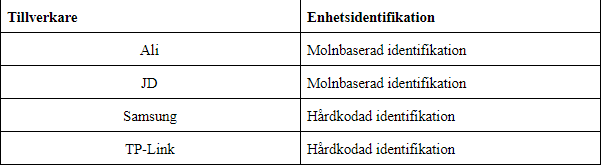
\includegraphics[width=8cm]{fig1.PNG}
    \caption{Tillverkare och metoder för identifikation[3]}
    \label{fig:Tabell 1}
\end{figure}


Man kan utnyttja ekosystemet genom att imitera smarthems enheter med en så kallad spökenhet [3].  En spökenhet är ett exekverbart program som imiterar en smarthems enhet. Den kan skicka information och kommandon till andra enheter i samma ekosystem. IoT enheter kan lätt imiteras. Detta då de bara använder en form av identifikation i form av enhetsidentifikation. Enhetsidentifikationen är olika beroende på tillverkare. I figur 1 visas ett par olika tillverkare och deras metod för enhets identifikation. Samsung använder till exempel ett hårdkodat enhets-id och asiatiska tillverkaren Ali delar ut ett enhets-id efter att enheterna paras ihop med deras molntjänster [3]. Därför finns det olika sätt att få tillgång till dessa. Samsungs är säkrast då man fysiskt behöver ha tillgång till enheten för att få tag i denna identifikation. Men detta kan lätt införskaffas genom att man fått sin enhet i andra hand. Till exempel ifall en förövare reklamerar en enhet efter att ha införskaffat sig enhetens identifikation[3]. Detta gör att enheten är utsatt i framtiden då identifikationen ej går att ändra på. Alis Alink har istället problemet att all deras källkod är öppen och man kan med detta jobba sig tillbaka till hur identifikationen skapas [3]. Med detta kan en förövare sedan skicka falsk data till molntjänsterna, som i sin tur kan leda till en rad olika problem för användare.

\begin{figure}[htp]
    \centering
    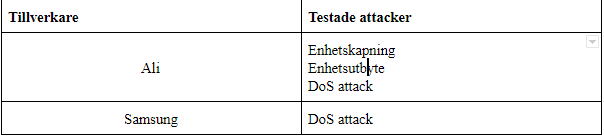
\includegraphics[width=8cm]{fig2.PNG}
    \caption{Tillverkare och attackmetoder[3]}
    \label{fig:Tabell 2}
\end{figure}

När en förövare kommit över information om en enhet i hemmet utgör detta stora risker för ens hem. Förövaren kan använda detta till att utföra en rad olika attacker. Vanliga sätt att attackera enheterna är till exempel enhetskapning, enhetsutbyte eller DoS attacker på enheten [3]. Dessa tre typer av attacker kan användas till en förövares fördel för att få tillgång till information som ej ska nås. I Figur 2 visas vilka olika typer av attacker som är testade per tillverkare.   Attackerna kan också användas för att förändra saker i hemmet. Lampor kopplade till ett IoT hem kan stängas av, eluttag kan avaktiveras eller kameror kan sluta användas. 

\section{Protokoll för det smarta hemmet}
%Förslag (Tristan)

Protokollen för smarthemmet kan ha ett flertal funktioner men har valts att diskuteras utifrån deras säkerhetsaspekter. Bland de utvalda IoT protokollen som man ser i Figur 3 (KNX-RF, ZigBee, Thread och Z-Wave) är var och en av dessa på olika lager enligt OSI-modellen och TCP/IP-modellen [7]. Dessutom fungerar protokollen olika beroende på hur topologin ser ut för dess enheter i det trådlösa utrymmet. Alla protokollen använder sig av någon form av AES (Authenticated Encryption Standard [14], en standardiserad krypteringsalgoritm som består av ett symmetriskt blockchiffer vilken kan kryptera och dekryptera information). 


\begin{figure}[htp]
    \centering
    \includegraphics[width=8cm]{komsysgrupparb.png}
    \caption{Protokoll för IoT, med alternativen för smarthem-enheter markerade i fetstil bortsett från EnOcean [7]}
    \label{fig:bild}
\end{figure}

\subsection{KNX}
KNX fokuserar sig på bland annat områden inom värme, ventilation och ljussättning i hem eller på arbetsplatser [7][8]. Protokollets förlängning KNX Data Security tillför de nödvändiga säkerhetsfunktionerna som autentisering, kryptering och dataintegritet med hjälp av AES-CCM (AES i CCM-läge [15], krypteringsalgoritm som bidrar med autentisering och konfidentialitet). Krypteringsalgoritmen fungerar som sådan att utbytet av hemliga nycklar sker med en projektspecifik nyckel som kommer från en FDSK (Factory Default Set up Key, en enhetsunik nyckel som inte kan ändras eller raderas) som är en gemensam statisk nyckel (Pre-Shared Key, en delad nyckel som bara är känd till sändare och mottagare sedan innan) [9][1].

\subsection{ZigBee}
ZigBee bygger på en IEEE standard och förlitar sig också på AES-CCM för sin kryptering och autentisering [7][10]. Detta protokoll kommer med inbyggda specifikationer för olika scenarion, till exempel ZigBee LightLink som används för smarthem produkter som är relaterade till ljus. ZigBee-nätverkssäkerhet förlitar sig på dess krypteringsnycklar varav det finns två typer [1][11]. Nätverksnyckeln är delad med alla enheter i nätverket och används för att säkra broadcast-kommunikation. Länknyckeln är bara delad mellan två enheter och används för att säkra unicast-kommunikation (mellan en sändare och en mottagare). Nycklarna blir utdelade antingen genom att de är pre-shared eller med hjälp av ett trust center (kan auktorisera nya enheter och hantera nyckeldistribution). Då nyckeln skapas med ett trust center finns det en chans att det måste ske okrypterat vilket riskerar en tillfällig sårbarhet. För IoT-enheter på lägre priser kan vissa inte hålla sina nycklar säkra på ett effektivt sätt så det blir svårare att hämta nätverksnycklar. 

\subsection{Thread}
Thread fungerar på nätverk i alla storlekar med enheter som har lite drivkraft [7][12]. Detta protokoll använder en nyckel som används över hela nätverket för att säkra paket med AES-CCM. Då denna nyckel är känd av alla enheter används också protokollen TLS (Transport Layer Security) och DTLS (Datagram Transport Layer Security) på applikationslagret som utrustar enheterna med fulla säkerhetstjänster. Problemet visas då protokollen används på enklare enheter, detta kan påverka deras prestanda negativt då de inte är byggda för den komplexiteten. Om en enhet blir utsatt kan det i sin tur utsätta hela nätverket, eller delar av det, för fara [7].

\subsection{Z-Wave}
Z-Wave inriktar sig på lättare trådlös och transmissiondata med mindre latens [7][13]. Inom sina Security Command Classes på sitt säkerhetslager finns S0 (Security 0) och S2 (Security 2) varav den senare är fokuserad på starkare säkerhet [7]. S2 använder AES-128 kryptering och ECDH (Elliptic Curve Diffie Hellman) systemet för att säkra nyckelutbytning. För S0 använder alla enheter samma nätverksnyckel (likt ZigBee), dock gör inte S2 detta utan låter alla subklasser sköta sina egna nätverk för att hindra att en enhet med mindre säkerhetsfunktioner som blivit utsatt skulle påverka klasser med högre säkerhet (problemet i Thread).


\section{Integritetsproblem}
%Integritetsproblem (Jacob)
Säker dataöverföring med skräddarsydda protokoll löser de viktigaste säkerhetsproblemen med smarthemmets IoT-enheter; däremot hanterar de inte alla integritetsproblem som uppstår då information om ens hem skickas över nätet. Som tidigare etablerat skickar få av dagens IoT-protokoll sin data utan kryptering, vilket innebär att det exakta innehållet i datan är oåtkomlig för utomstående parter som inte har tillgång till krypteringsnyckeln. Vad som kan orsaka integritetsproblem med smarthemmets IoT ligger därmed i den grundläggande principen för nätbaserad kommunikation snarare än i de moderna protokoll och överföringsmetoder som används för de flesta av dagens IoT-enheter. Som nätbaserad kommunikation är uppbyggd idag finns information om sändare, mottagare, datans storlek och tidpunkten för överföringen publikt tillgänglig för alla som kan avläsa den överförda datan även om den är krypterad. Sådan information har sällan tidigare varit känslig, men för smarthemsenheter, som skickar information om en specifik process i ett specifikt hem till en specifik server vid specifika tidpunkter kan den användas för att analysera och dra slutsatser om vad de boende i hemmet gör [7]. 

[2] undersökte dataflödet hos några av de mest populära smarthemsenheterna på marknaden, däribland en sömnmätare från Sense, en inomhuskamera från Nest och röstassistenten Echo från Amazon. Genom att installera enheterna i en miljö som simulerade ett riktigt hem och avläsa deras datatrafik i hemmets router, likt hur en ISP kan göra, undersökte de om känslig information kunde avläsas från datatrafiken. De fann att datatrafiken hos samtliga enheter endast uppstod eller ökade kraftigt när de registrerade information från hemmet. Därtill skickade enheterna sin information till domännamn som tydligt tillhörde deras företag, vilket innebar att enheterna kunde identifieras från enbart sin datatrafik. Utifrån dessa insikter och den insamlade datan kunde de dra slutsatser om när den boende i hemmet somnade och vaknade, passerade inomhuskameran och pratade med röstassistenten utan att behöva nå den krypterade datan. 


\section{Avslutning}
Avslutningsvis finns vissa säkerhets- och integritetsrisker kvar med IoT-enheter i hemmet trots den ökade försäljningen av dem. Exempel på generella säkerhetshot som nämns i rapporten är obehöriga användare som får tillgång till nätverket i hemmet, hårdvarubegränsningar och uppdateringar i IoT-enheter samt problematiken med olika nätverksstandarder hos enheterna.

Ytterligare ett säkerhetshot med smarthemsenheter är spökenheter. Dessa kan utnyttja det smarta hemmets ekosystem genom att imitera IoT enheter. Spökenheterna kan skicka olika typer av kommandon mellan det smarta molnet och andra smarthemsenheter. Detta gör att spökenheterna kan interagera med ekosystemet på oönskade och oförutsägbara sätt. Sensorer kan skicka fel data vilket sedan kan leda till olika konsekvenser beroende på hur ens system är konfigurerat.

En lösning på säkerhetsriskerna med smart hemmet kan vara nya och bättre anpassade protokoll. I rapporten har några av de största smarthemsspecifika protokollen beskrivits. Alla nämnda protokoll använde i princip olika former av samma nyckelsalgoritm. Thread använder protokollet TLS för att kompensera för användningen av symmetriska nycklar, som däremot får nackdelen att prestandan för enheter med lägre beräkningskraft blir sämre. Av de utvalda protokollen hade Z-Wave starkast uppbyggnad med S0, S2 och deras underkategorier. 

Även om dessa protokoll medför högre säkerhet så löser de inte integritetsproblem som redan nu visats möjliga. Genom att analysera dataflödet hos flera smarthemsenheter har integriteten hos deras information visats sårbar, trots att datan är krypterad. Detta kan potentiellt utnyttjas för att skapa en bild av vad som pågår i hemmet. 

% You must have at least 2 lines in the paragraph with the drop letter
% (should never be an issue)


% An example of a floating figure using the graphicx package.
% Note that \label must occur AFTER (or within) \caption.
% For figures, \caption should occur after the \includegraphics.
% Note that IEEEtran v1.7 and later has special internal code that
% is designed to preserve the operation of \label within \caption
% even when the captionsoff option is in effect. However, because
% of issues like this, it may be the safest practice to put all your
% \label just after \caption rather than within \caption{}.
%
% Reminder: the "draftcls" or "draftclsnofoot", not "draft", class
% option should be used if it is desired that the figures are to be
% displayed while in draft mode.
%
%\begin{figure}[!t]
%\centering
%\includegraphics[width=2.5in]{myfigure}
% where an .eps filename suffix will be assumed under latex, 
% and a .pdf suffix will be assumed for pdflatex; or what has been declared
% via \DeclareGraphicsExtensions.
%\caption{Simulation results for the network.}
%\label{fig_sim}
%\end{figure}

% Note that the IEEE typically puts floats only at the top, even when this
% results in a large percentage of a column being occupied by floats.


% An example of a double column floating figure using two subfigures.
% (The subfig.sty package must be loaded for this to work.)
% The subfigure \label commands are set within each subfloat command,
% and the \label for the overall figure must come after \caption.
% \hfil is used as a separator to get equal spacing.
% Watch out that the combined width of all the subfigures on a 
% line do not exceed the text width or a line break will occur.
%
%\begin{figure*}[!t]
%\centering
%\subfloat[Case I]{\includegraphics[width=2.5in]{box}%
%\label{fig_first_case}}
%\hfil
%\subfloat[Case II]{\includegraphics[width=2.5in]{box}%
%\label{fig_second_case}}
%\caption{Simulation results for the network.}
%\label{fig_sim}
%\end{figure*}
%
% Note that often IEEE papers with subfigures do not employ subfigure
% captions (using the optional argument to \subfloat[]), but instead will
% reference/describe all of them (a), (b), etc., within the main caption.
% Be aware that for subfig.sty to generate the (a), (b), etc., subfigure
% labels, the optional argument to \subfloat must be present. If a
% subcaption is not desired, just leave its contents blank,
% e.g., \subfloat[].


% An example of a floating table. Note that, for IEEE style tables, the
% \caption command should come BEFORE the table and, given that table
% captions serve much like titles, are usually capitalized except for words
% such as a, an, and, as, at, but, by, for, in, nor, of, on, or, the, to
% and up, which are usually not capitalized unless they are the first or
% last word of the caption. Table text will default to \footnotesize as
% the IEEE normally uses this smaller font for tables.
% The \label must come after \caption as always.
%
%\begin{table}[!t]
%% increase table row spacing, adjust to taste
%\renewcommand{\arraystretch}{1.3}
% if using array.sty, it might be a good idea to tweak the value of
% \extrarowheight as needed to properly center the text within the cells
%\caption{An Example of a Table}
%\label{table_example}
%\centering
%% Some packages, such as MDW tools, offer better commands for making tables
%% than the plain LaTeX2e tabular which is used here.
%\begin{tabular}{|c||c|}
%\hline
%One & Two\\
%\hline
%Three & Four\\
%\hline
%\end{tabular}
%\end{table}


% Note that the IEEE does not put floats in the very first column
% - or typically anywhere on the first page for that matter. Also,
% in-text middle ("here") positioning is typically not used, but it
% is allowed and encouraged for Computer Society conferences (but
% not Computer Society journals). Most IEEE journals/conferences use
% top floats exclusively. 
% Note that, LaTeX2e, unlike IEEE journals/conferences, places
% footnotes above bottom floats. This can be corrected via the
% \fnbelowfloat command of the stfloats package.




% conference papers do not normally have an appendix


% use section* for acknowledgment





% trigger a \newpage just before the given reference
% number - used to balance the columns on the last page
% adjust value as needed - may need to be readjusted if
% the document is modified later
%\IEEEtriggeratref{8}
% The "triggered" command can be changed if desired:
%\IEEEtriggercmd{\enlargethispage{-5in}}

% references section

% can use a bibliography generated by BibTeX as a .bbl file
% BibTeX documentation can be easily obtained at:
% http://mirror.ctan.org/biblio/bibtex/contrib/doc/
% The IEEEtran BibTeX style support page is at:
% http://www.michaelshell.org/tex/ieeetran/bibtex/
%\bibliographystyle{IEEEtran}
% argument is your BibTeX string definitions and bibliography database(s)
%\bibliography{IEEEabrv,../bib/paper}
%
% <OR> manually copy in the resultant .bbl file
% set second argument of \begin to the number of references
% (used to reserve space for the reference number labels box)
\begin{thebibliography}{1}

% RÄTTA REFERENSER LIGGER I UTKAST V2

  \bibitem{IEEEhowto:kopka}
N. Apthorpe, D. Reisman, S. Sundaresan, A. Narayanan, N. Feamster, Spying on the Smart Home: Privacy Attacks and Defenses on Encrypted IoT Traffic, 2017
 %vart kommer 10an i början från?
  \bibitem{IEEEhowto:kopka}
N. Apthorpe, D. Reisman, N. Feamster, A Smart Home is No Castle: Privacy Vulnerabilities of Encrypted IoT Traffic, Computer Science Dept. Princeton University, 2017
  
  \bibitem{IEEEhowto:kopka}
W. Zhou, Y. Jia, Y. Yao, L. Zhu, L. Guan, Y. Mao, P. Liu, Y. Zhang, Discovering and Understanding the Security Hazards in the Interactions between IoT Devices, Mobile Apps, and Clouds on Smart Home Platforms, National Computer Network Intrusion Protection Center, University of Chinese Academy of Sciences (China), School of Cyber Engineering, Xidian University (China), Department of Computer Science, University of Georgia (USA),  College of Information Sciences and Technology, The Pennsylvania State University (USA), State Key Laboratory of Information Security, Institute of Information Engineering, Chinese Academy of Sciences (China), 2019

  \bibitem{IEEEhowto:kopka}
Statista. Smart Home Market, https://www.statista.com/outlook/279/154/smart-home/sweden (Hämtad: 2019-10-06)
  
  \bibitem{IEEEhowto:kopka}
C-C. Teng, J-W. Gong, Y-S. Wang, C-P. Chuang, M-C. Chen, Firmware over the air for home cybersecurity in the Internet of Things, Network Management Laboratory, Chunghwa Telecom Laboratories Co., Ltd., Taoyuan, Taiwan, R.O.C., 2017
  
  \bibitem{IEEEhowto:kopka}
V. Hedtjärn Swaling, J. Johansson, NCS3 Studie – IoT-relaterade risker och strategier Risker relaterade till Internet of Things (IoT) och vad myndigheter kan göra för att motverka dem, FOI-R--4591--SE, MSB 2017-1554, ISSN 1650-1942, 2018
  
  \bibitem{IEEEhowto:kopka}
S. Marksteiner, V. J. Exposito Jiménez, H. Vallant, and H. Zeiner, An Overview of Wireless IoT Protocol Security in the Smart Home Domain, \emph{2017 Joint 13th CTTE and 10th CMI Conference on Internet of Things Business Models, Users, and Networks}, Copenhagen, 2017, pp. 1-8. doi: 10.1109/CTTE.2017.8260940., JOANNEUM RESEARCH Forschungsgesellschaft mbH, DIGITAL - Institute for Information and Communication Technologies


  \bibitem{IEEEhowto:kopka}
KNX Association, https://www.knx.org/ (Hämtad: 2019-10-06)

  \bibitem{IEEEhowto:kopka}
  KNX Association, KNX Secure, KNX Position Paper on Data Security and Privacy, https://www.knx.org/wAssets/docs/downloads/Marketing/Flyers/KNX-Secure-Position-Paper/KNX-Secure-Position-Paper\_en.pdf (Hämtad: 2019-10-06)


  \bibitem\IEEEtriggeratref{10}.
ZigBee Alliance, https://www.zigbee.org/ (Hämtad: 2019-10-06)

  \bibitem{IEEEhowto:kopka}
T. Zillner, ZigBee Exploited - The good, the bad and the ugly, in Presented as part of the \emph{BlackHat 2015 Conference}. Las Vegas, NV: Blackhat, 2015. 

  \bibitem{x}
Thread Group, https://www.threadgroup.org/ (Hämtad: 2019-10-06) 

  \bibitem{x}
Z-Wave Alliance, https://z-wavealliance.org/ (Hämtad: 2019-10-06)

  \bibitem{x}
Federal Information Processing Standards Publication 197, Announcing the Advanced Encryption Standard (AES), 2001

  \bibitem{x}
M. Dworkin, Recommendation for Block Cipher Modes of Operation: The CCM Mode for Authentication and Confidentiality, NIST Special Publication 800-38C, 2004, uppdaterad 2007

\end{thebibliography}



% that's all folks
\end{document}


